% This is samplepaper.tex, a sample chapter demonstrating the
% LLNCS macro package for Springer Computer Science proceedings;
% Version 2.20 of 2017/10/04
%
\documentclass[runningheads]{llncs}
%
\usepackage{graphicx}
% Used for displaying a sample figure. If possible, figure files should
% be included in EPS format.
%
% If you use the hyperref package, please uncomment the following line
% to display URLs in blue roman font according to Springer's eBook style:
% \renewcommand\UrlFont{\color{blue}\rmfamily}

\begin{document}
%
\title{Contribution Title\thanks{Supported by organization x.}}
%
%\titlerunning{Abbreviated paper title}
% If the paper title is too long for the running head, you can set
% an abbreviated paper title here
%
\author{First Author\inst{1}\orcidID{0000-1111-2222-3333} \and
Second Author\inst{2,3}\orcidID{1111-2222-3333-4444} \and
Third Author\inst{3}\orcidID{2222--3333-4444-5555}}
%
\authorrunning{F. Author et al.}
% First names are abbreviated in the running head.
% If there are more than two authors, 'et al.' is used.
%
\institute{University of Salento, Lecce Le 73100, IT \and
Springer Heidelberg, Tiergartenstr. 17, 69121 Heidelberg, Germany
\email{lncs@springer.com}\\
\url{http://www.springer.com/gp/computer-science/lncs} \and
ABC Institute, Rupert-Karls-University Heidelberg, Heidelberg, Germany\\
\email{\{abc,lncs\}@uni-heidelberg.de}}
%
\maketitle              % typeset the header of the contribution
%
\begin{abstract}
The abstract should briefly summarize the contents of the paper in
150--250 words.

\keywords{Plant Phenotyping  \and Instance Segmentation \and Object Detection.}
\end{abstract}
%
%
%
\clearpage

\section{Introduction}
High throughput plant phenotyping is one of the most complicated and time expensive challenge of this day. Nowadays cameras are getting
involved in many fields. Manually look along each plant and each component takes a long of time, cameras can be helpful in order to improve
speed of control and it's accuracy. With only RGB 2D images spatial information can be extrapolated and some spectral ones. With 3D ones instead,
crucial information can be discovered such as: dimensions, height, weight. In order to measure this phenotyping traits we need more than one computer
vision task, locate a plant with object detection, segment single leaf with instance or semantic segmentation, where deep learning techniques can provide
general and precise data \cite{CNN_HTPP_R}.

Morphological changes are a crucial aspect of plant growth, leaf area and leaf height are commonly used to understand how plant is changing during time.
Using only RGB images can be hard to extrapolate this information due to environmental light, shades and so on. CNNs are widely used in this field obtaining
great results. Teimouri, Dyrmann, Nielsen, Mathiassen, Somerville and Jørgensen \cite{weedestimator}, tried to count leaves in 18 different species, in order to
do this they used deep CNNs and trained them with a lot of images. They have used Inception-v3 \cite{inceptionv3} architecture for its good performance.
In a second time the authors tried to predict growth stage of plants and they have found that with more plants in the same image the accuracy is worst. With the
Inception-v3 they obtained an accuracy by 83\%, with a count estimation typically overestimated.
Bhugra, Garg, Chaudhury, and Lall, in order to analyze shape variation, have created a new methodology to segment each leaf instance. To avoid scene variability
they have used Mean-shift \cite{meanshift} Bandwidths Searching Latent Dirichlet Allocation. To enhance the results given by Mean-Shift the authors have employed the
distance between texture descriptors, then they nominate leaf candidate so leaf representative can be extracted. Masks can be finally created and different approaches
for estimate if a leaf is a non-overlapped ones are used. Gaussian Mixture Models was found to be noisy while different method like Minervini's algorithm K-means and
Otsu's threshold overestimate the foreground giving disconnected regions. Instead Two approaches based on Mean-Shift, using the orientation field map and a
polar transformation of the leaf tips, done with Harris-Stephens angle detector. While the second, starts from the polar transformed images, from which skeletal image
is taken. This kind of approaches oversegment non-overlapped leaves but has a good ground truth for the corresponding ones. Based on Plant phenotyping images database,
the authors obtained a DICE score map of 89.9\% \cite{DICE}.
In Fine-grained recognition in high-throughput phenotyping \cite{FGrecognition} the authors aimed to classify the single plant inside the cultivars. In order to do that,
all plants of the dataset were divided into different growth stages, then they have localized the plants with a prior knowledge and after that the authors have segmented the
same with Otsu's threshold or green based brightness. Data were post-processed with different methods. Radial Object Descriptors are completed
with ResNet18 \cite{ResNet18} and Histogram of Oriented Gradients with Softmax regression. They have tested different combination of this methods and have analyzed
the results with for mean accuracy, which aims to analyze the goodness of classification. ROD-HOD-Softmax outperforms the ResNet18 method in one of the four dataset
used, and only in the early stages, but the gap is lower when the plants start growing. Instead for the remaining three datasets, the combination of resnet with
the radial object descriptor outperforms the histogram of oriented gradients.







% \subsection{A Subsection Sample}
% Please note that the first paragraph of a section or subsection is
% not indented. The first paragraph that follows a table, figure,
% equation etc. does not need an indent, either.

% Subsequent paragraphs, however, are indented.

% \subsubsection{Sample Heading (Third Level)} Only two levels of
% headings should be numbered. Lower level headings remain unnumbered;
% they are formatted as run-in headings.

% \paragraph{Sample Heading (Fourth Level)}
% The contribution should contain no more than four levels of
% headings. Table~\ref{tab1} gives a summary of all heading levels.

% \begin{table}
% \caption{Table captions should be placed above the
% tables.}\label{tab1}
% \begin{tabular}{|l|l|l|}
% \hline
% Heading level &  Example & Font size and style\\
% \hline
% Title (centered) &  {\Large\bfseries Lecture Notes} & 14 point, bold\\
% 1st-level heading &  {\large\bfseries 1 Introduction} & 12 point, bold\\
% 2nd-level heading & {\bfseries 2.1 Printing Area} & 10 point, bold\\
% 3rd-level heading & {\bfseries Run-in Heading in Bold.} Text follows & 10 point, bold\\
% 4th-level heading & {\itshape Lowest Level Heading.} Text follows & 10 point, italic\\
% \hline
% \end{tabular}
% \end{table}


% \noindent Displayed equations are centered and set on a separate
% line.
% \begin{equation}
% x + y = z
% \end{equation}
% Please try to avoid rasterized images for line-art diagrams and
% schemas. Whenever possible, use vector graphics instead (see
% Fig.~\ref{fig1}).

% \begin{figure}
% 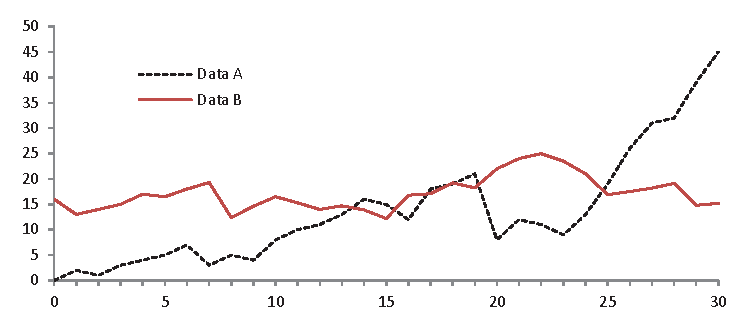
\includegraphics[width=\textwidth]{fig1.eps}
% \caption{A figure caption is always placed below the illustration.
% Please note that short captions are centered, while long ones are
% justified by the macro package automatically.} \label{fig1}
% \end{figure}

% \begin{theorem}
% This is a sample theorem. The run-in heading is set in bold, while
% the following text appears in italics. Definitions, lemmas,
% propositions, and corollaries are styled the same way.
% \end{theorem}
% %
% % the environments 'definition', 'lemma', 'proposition', 'corollary',
% % 'remark', and 'example' are defined in the LLNCS documentclass as well.
% %
% \begin{proof}
% Proofs, examples, and remarks have the initial word in italics,
% while the following text appears in normal font.
% \end{proof}
% For citations of references, we prefer the use of square brackets
% and consecutive numbers. Citations using labels or the author/year
% convention are also acceptable. The following bibliography provides
% a sample reference list with entries for journal
% articles~\cite{ref_article1}, an LNCS chapter~\cite{ref_lncs1}, a
% book~\cite{ref_book1}, proceedings without editors~\cite{ref_proc1},
% and a homepage~\cite{ref_url1}. Multiple citations are grouped
% \cite{ref_article1,ref_lncs1,ref_book1},
% \cite{ref_article1,ref_book1,ref_proc1,ref_url1}.




%
% ---- Bibliography ----
%
% BibTeX users should specify bibliography style 'splncs04'.
% References will then be sorted and formatted in the correct style.
%
% \bibliographystyle{splncs04}
% \bibliography{mybibliography}
%
\begin{thebibliography}{8}
\bibitem{CNN_HTPP_R}
Author, Jiang Yu, Li Changying:
Convolutional Neural Networks for Image-Based High-Throughput Plant Phenotyping: A Review.
Plant Phenomics (2020)

\bibitem{inceptionv3}
Author, Szegedy, Christian and Vanhoucke, Vincent and Ioffe, Sergey and Shlens, Jon and Wojna, Zbigniew:
Rethinking the inception architecture for computer vision.
In: Proceedings of the IEEE conference on computer vision and pattern recognition, pp. 2818--2826 (2016) 

\bibitem{weedestimator}
Author, Teimouri, Nima and Dyrmann, Mads and Nielsen, Per Rydahl and Mathiassen, Solvejg Kopp and Somerville, Gayle J. and Jørgensen, Rasmus Nyholm:
Weed growth stage estimator using deep convolutional neural networks.
vol. 18, Sensors (2018)

\bibitem{meanshift}
Comaniciu, Dorin and Meer, Peter:
Mean shift: A robust approach toward feature space analysis.
In: IEEE Transactions on pattern analysis and machine intelligence, vol. 24 pp. 603--619, IEEE (2002)

\bibitem{DICE}
Authors, Scharr, H., Minervini, M., French, A. P., Klukas, C., Kramer, D. M., Liu, X., Tsaftaris: S. A. (2016). 
Leaf segmentation in plant phenotyping: a collation study.
In: Machine vision and applications, vol. 27 pp. 585--606, Springer (2016) 

\bibitem{FGrecognition}
Authors, Lyu, Beichen and Smith, Stuart D. and Cherkauer, Keith A.:
Fine-Grained Recognition in High-throughput Phenotyping.
In: 2020 IEEE/CVF Conference on Computer Vision and Pattern Recognition Workshops (CVPRW), pp. 320--329 IEEE (2020)

\bibitem{ResNet18}
Authors, He, Kaiming and Zhang, Xiangyu and Ren, Shaoqing and Sun, Jian:
Deep residual learning for image recognition
In: Proceedings of the IEEE conference on computer vision and pattern recognition,
pp 770--778, IEEE (2016)

% \bibitem{ref_lncs1}
% Author, F., Author, S.: Title of a proceedings paper. In: Editor,
% F., Editor, S. (eds.) CONFERENCE 2016, LNCS, vol. 9999, pp. 1--13.
% Springer, Heidelberg (2016). \doi{10.10007/1234567890}

% \bibitem{ref_book1}
% Author, F., Author, S., Author, T.: Book title. 2nd edn. Publisher,
% Location (1999)

% \bibitem{ref_proc1}
% Author, A.-B.: Contribution title. In: 9th International Proceedings
% on Proceedings, pp. 1--2. Publisher, Location (2010)

% \bibitem{ref_url1}
% LNCS Homepage, \url{http://www.springer.com/lncs}. Last accessed 4
% Oct 2017
\end{thebibliography}
\end{document}
